\chapter{座標変換と可視化}
\label{chap:tf_viz}

% この章で学ぶこと
\begin{goalbox}
  \begin{itemize}
    \item ロボットで使う座標系と、ROS 2 での座標系の決まり
    \item tf2 による座標変換のしくみと、それを調べるツール
    \item URDF を使ったロボットの形の書き方
    \item \cmd{robot\_state\_publisher} と \cmd{joint\_state\_publisher} の役割
    \item RViz2 を使ったロボットやセンサのデータの表示
  \end{itemize}
\end{goalbox}

ロボットは、自分の体のどこにセンサが付いていて、自分が部屋のどこにいるのかを知らなければ、うまく動けません。
たとえば、LiDAR が「前方 1 m に障害物がある」と測っても、その LiDAR がロボットの前の端に付いているのか、真ん中に付いているのかで、ロボットの本体から障害物までの距離は変わります。
この章では、ロボットの体や周りの世界の位置関係を扱う\textbf{座標変換}のしくみと、それを目で見て確かめるための可視化ツール RViz2 を学びます。

\section{ロボットにおける座標系}
\label{sec:tf-viz-frames}

\subsection{座標系とは}

位置や向きを数値で表すには、「どこを原点にして、どちらの向きを x・y・z にするか」を決める必要があります。
これを\textbf{座標系}（フレーム）といいます。
ロボットでは、1 つの座標系だけでなく、ロボットの本体・各センサ・地図など、たくさんの座標系を使います。
同じ障害物でも、LiDAR の座標系で見た位置と、ロボットの本体の座標系で見た位置は違う値になります。
ある座標系で表した位置を、別の座標系での位置に直すことを\textbf{座標変換}といいます。

\subsection{ROS 2 の座標系の決まり}

ROS 2 では、座標系の向きと単位について、次のような決まりがあります（REP 103 という文書で決められています）。

\begin{itemize}
  \item ロボットの座標系は、\textbf{x 軸が前、y 軸が左、z 軸が上}（図\ref{fig:tf-viz-axes}）
  \item 長さの単位はメートル [m]、角度の単位はラジアン [rad]、時間の単位は秒 [s]
  \item 回転は、軸の向きに右手の親指を向けたとき、ほかの指が曲がる向きが正（z 軸まわりなら、上から見て左回りが正）
\end{itemize}

\begin{figure}[tb]
  \centering
  % 図：ロボットの座標系の向き（chapters/ros2/tf_viz.tex）
\begin{tikzpicture}[ax/.style={-{Stealth[length=2.2mm]}, very thick}]
  % 上から見た図
  \begin{scope}
    \draw[rounded corners=3pt, fill=blue!8] (-1.1,-0.75) rectangle (1.1,0.75);
    \fill[black!70] (-0.45,0.75) rectangle (0.45,0.95);
    \fill[black!70] (-0.45,-0.95) rectangle (0.45,-0.75);
    \draw[ax, red!80!black] (0,0) -- (1.9,0) node[right]{$x$（前）};
    \draw[ax, green!50!black] (0,0) -- (0,1.7) node[above]{$y$（左）};
    \fill (0,0) circle (1.5pt);
    \node[figlabel, below] at (0,-1.1) {上から見た図（$z$ は手前向き＝上）};
    \draw[-{Stealth[length=1.8mm]}, thick, orange!80!black] (0.75,0.25) arc (20:110:0.8);
    \node[figlabel, orange!80!black, anchor=east] at (-0.3,1.3) {$z$ 軸まわりの回転\\（ヨー、左回りが正）};
  \end{scope}
  % 横から見た図
  \begin{scope}[xshift=6.3cm]
    \draw[rounded corners=3pt, fill=blue!8] (-1.1,0.1) rectangle (1.1,0.8);
    \draw[fill=black!70] (0,0.1) circle (0.28);
    \draw[ax, red!80!black] (0,0.45) -- (1.9,0.45) node[right]{$x$（前）};
    \draw[ax, blue!70!black] (0,0.45) -- (0,2.0) node[above]{$z$（上）};
    \fill (0,0.45) circle (1.5pt);
    \draw[thick] (-1.6,-0.18) -- (2.0,-0.18);
    \node[figlabel, below] at (0,-0.35) {横から見た図（$y$ は奥向き＝左）};
  \end{scope}
\end{tikzpicture}

  \caption{ロボットの座標系の向き}
  \label{fig:tf-viz-axes}
\end{figure}

z 軸まわりの回転を\textbf{ヨー}（yaw）、y 軸まわりを\textbf{ピッチ}（pitch）、x 軸まわりを\textbf{ロール}（roll）といいます。
平面を走る移動ロボットでは、主にヨー（ロボットがどちらを向いているか）を使います。
\ref{sec:ros2-concepts-topic}節の \cmd{Twist} で、\cmd{linear.x} が前後の速度、\cmd{angular.z} が回転の速度だったのも、この決まりに従っているからです。

\subsection{移動ロボットの座標系}

移動ロボットでは、次のような名前の座標系がよく使われます（図\ref{fig:tf-viz-frame-tree}）。

\begin{description}
  \item[\cmd{base\_link}] ロボットの本体に固定された座標系です。ロボットが動くと、一緒に動きます。
  \item[\cmd{laser}, \cmd{camera\_link} など] センサや部品に固定された座標系です。\cmd{base\_link} から見た取り付け位置で決まります。
  \item[\cmd{odom}] ロボットが動き始めた位置を原点とする座標系です。車輪の回転などから計算した移動量（\textbf{オドメトリ}）で、\cmd{odom} から見た \cmd{base\_link} の位置がわかります。ただし、車輪のすべりなどで、だんだんずれていきます。
  \item[\cmd{map}] 地図に固定された座標系です。地図とセンサのデータを照らし合わせて（\ref{sec:practice-slam}節）、オドメトリのずれを補正します。
\end{description}

\begin{figure}[tb]
  \centering
  % 図：移動ロボットの座標系のつながり（chapters/ros2/tf_viz.tex）
\begin{tikzpicture}[fr/.style={draw, rounded corners=2pt, font=\small\ttfamily, minimum width=24mm, minimum height=7mm, fill=blue!6},
    note/.style={font=\scriptsize, align=left, text=black!70, anchor=west}]
  \node[fr] (map) at (0,0) {map};
  \node[fr] (odom) at (0,-1.4) {odom};
  \node[fr] (base) at (0,-2.8) {base\_link};
  \node[fr] (laser) at (-3.2,-4.3) {laser};
  \node[fr] (camera) at (0,-4.3) {camera\_link};
  \node[fr] (wheel) at (3.2,-4.3) {left\_wheel など};
  \draw[figarrow] (map) -- (odom);
  \draw[figarrow] (odom) -- (base);
  \draw[figarrow] (base) -- (laser);
  \draw[figarrow] (base) -- (camera);
  \draw[figarrow] (base) -- (wheel);
  \node[note] at (1.5,0) {地図の座標系（世界に固定）};
  \node[note] at (1.5,-0.7) {SLAM や自己位置推定が求める（ずれを補正する）};
  \node[note] at (1.5,-1.4) {動き始めた位置の座標系};
  \node[note] at (1.5,-2.1) {車輪の回転などから求める（だんだんずれる）};
  \node[note] at (1.5,-2.8) {ロボットの本体の座標系};
  \node[note] at (-4.4,-5.05) {センサや部品の座標系（URDF に書いた取り付け位置で決まる）};
\end{tikzpicture}

  \caption{移動ロボットの座標系のつながり}
  \label{fig:tf-viz-frame-tree}
\end{figure}

座標系どうしは、図のように親と子の関係でつながった木の形（\textbf{ツリー}）になっています。
つながっていれば、どの 2 つの座標系の間でも、途中の座標変換を順にたどって、位置を変換できます。

\section{tf2 の仕組み}
\label{sec:tf-viz-tf2}

\subsection{tf2 とは}

ROS 2 では、座標系どうしの位置関係を、\textbf{tf2} というしくみで管理します。
各ノードは、「親の座標系から見た、子の座標系の位置と向き」を、\cmd{/tf} と \cmd{/tf\_static} という 2 つのトピックにパブリッシュします。
座標変換を使いたいノードは、これらのトピックをサブスクライブしておき、必要なときに「A の座標系から見た B の座標系の位置」を問い合わせます。
途中の変換をたどる計算は、tf2 がやってくれます。

\begin{tablebox}[tf2 の 2 つのトピック][tab:tf-viz-topics]
  \begin{tabular}{lp{0.6\linewidth}}
    \toprule
    トピック & 流すもの \\
    \midrule
    \cmd{/tf} & 時間とともに変わる座標変換（\cmd{odom} → \cmd{base\_link}、車輪の回転など）。何度もパブリッシュし続ける \\
    \cmd{/tf\_static} & 変わらない座標変換（\cmd{base\_link} → \cmd{laser} など、ねじで固定されたセンサの位置）。1 回だけパブリッシュする \\
    \bottomrule
  \end{tabular}
\end{tablebox}

\subsection{turtlesim で tf2 を試す}

ROS 2 には、turtlesim を使った tf2 のデモが用意されています。
必要なパッケージをインストールして、起動してみましょう。

\begin{terminal}[tf2 のデモをインストールして起動する]
$ sudo apt install ros-jazzy-turtle-tf2-py ros-jazzy-tf2-tools
$ ros2 launch turtle_tf2_py turtle_tf2_demo.launch.py
\end{terminal}

turtlesim のウィンドウに 2 匹のカメが現れます。
別のターミナルで \cmd{turtle\_teleop\_key} を起動して 1 匹目のカメを動かすと、2 匹目のカメが後を追いかけてきます。

\begin{terminal}[1 匹目のカメを動かす]
$ ros2 run turtlesim turtle_teleop_key
\end{terminal}

このデモでは、それぞれのカメの位置が、\cmd{world} 座標系から見た \cmd{turtle1} 座標系、\cmd{turtle2} 座標系として、\cmd{/tf} にパブリッシュされています。
追いかけるノードは、tf2 に「\cmd{turtle2} から見た \cmd{turtle1} の位置」を問い合わせ、その方向に進むように速度の指令を送っています。

\subsection{座標変換を調べるツール}

座標変換を調べるためのツールが、いくつか用意されています。
\cmd{tf2\_echo} は、2 つの座標系の間の座標変換を表示し続けます。

\begin{terminal}[2 つの座標系の間の座標変換を表示する]
$ ros2 run tf2_ros tf2_echo world turtle1
At time 1727852400.123456789
- Translation: [5.544, 5.544, 0.000]
- Rotation: in Quaternion (xyzw) [0.000, 0.000, 0.000, 1.000]
- Rotation: in RPY (radian) [0.000, -0.000, 0.000]
- Rotation: in RPY (degree) [0.000, -0.000, 0.000]
...
\end{terminal}

\cmd{Translation} が位置（x, y, z）、\cmd{Rotation} が向きです。
向きは、ロール・ピッチ・ヨー（RPY）のほかに、\textbf{クォータニオン}という 4 つの数（x, y, z, w）でも表示されています。
クォータニオンは、計算機で回転を扱うのに便利な表し方で、ROS 2 のメッセージの中では、向きはクォータニオンで表されます。
中身を理解できなくても、ライブラリが RPY との変換をしてくれるので、はじめのうちは「向きはクォータニオンで表される」とだけ覚えておけば十分です。

\cmd{view\_frames} を使うと、座標系のつながりを図にした PDF ファイルを作れます。

\begin{terminal}[座標系のつながりを PDF にする]
$ ros2 run tf2_tools view_frames
...
$ ls frames_*.pdf
frames_2026-10-02_10.00.00.pdf
\end{terminal}

\subsection{固定された座標変換をパブリッシュする}

ロボットにセンサを取り付けたときなど、変わらない座標変換をパブリッシュしたいときは、\cmd{static\_transform\_publisher} を使います。
たとえば、本体（\cmd{base\_link}）の中心から前に 0.1 m、上に 0.2 m の位置に LiDAR（\cmd{laser}）を取り付けた場合は、次のように実行します。

\begin{terminal}[固定された座標変換をパブリッシュする]
$ ros2 run tf2_ros static_transform_publisher --x 0.1 --y 0 --z 0.2 --yaw 0 --pitch 0 --roll 0 --frame-id base_link --child-frame-id laser
\end{terminal}

ただし、ロボットの部品の取り付け位置は、次の節の URDF にまとめて書いておくのが一般的です。

\subsection{プログラムから座標変換を使う}

自分のノードで座標変換を使うときは、\cmd{tf2\_ros} パッケージを使います。
次のノードは、tf2 のデモが動いている状態で、\cmd{world} 座標系から見た \cmd{turtle1} の位置を 1 秒ごとに表示します。

\codefile[style=python, firstline=10, lastline=27]{座標変換を調べるノード（my\_package/frame\_listener.py）}{lst:tf-viz-listener}{samples/rclpy/my_package/my_package/frame_listener.py}

\cmd{Buffer} は、届いた座標変換をためておく入れ物で、\cmd{TransformListener} が \cmd{/tf} と \cmd{/tf\_static} をサブスクライブして、\cmd{Buffer} に入れてくれます。
\cmd{lookup\_transform(親, 子, 時刻)} で、座標変換を問い合わせます。
時刻に \cmd{Time()} を指定すると、最新の座標変換が得られます。
起動したばかりで、まだ座標変換が届いていないときは例外（\ref{sec:python-class-exception}節）が起きるので、\cmd{try} で受け止めています。

\section{URDF によるロボットモデルの記述}
\label{sec:tf-viz-urdf}

\subsection{URDF とは}

\textbf{URDF}（Unified Robot Description Format）は、ロボットの形や、部品のつながりを書くための、XML の形式のファイルです。
URDF では、ロボットを\textbf{リンク}と\textbf{ジョイント}の組み合わせで表します。

\begin{description}
  \item[リンク（link）] ロボットの部品（本体、車輪、センサなど）です。見た目の形や大きさ、色などを書きます。リンクごとに、同じ名前の座標系ができます。
  \item[ジョイント（joint）] 2 つのリンクのつなぎ目（関節）です。親のリンクから見た子のリンクの位置と、どのように動くかを書きます。
\end{description}

ジョイントには、次のような種類があります。

\begin{tablebox}[ジョイントの主な種類][tab:tf-viz-joints]
  \begin{tabular}{lp{0.6\linewidth}}
    \toprule
    種類 & 動き方 \\
    \midrule
    \cmd{fixed} & 動かない（ねじで固定されたセンサなど） \\
    \cmd{continuous} & 軸のまわりに、制限なく回転する（車輪など） \\
    \cmd{revolute} & 軸のまわりに、決まった角度の範囲で回転する（アームの関節など） \\
    \cmd{prismatic} & 軸に沿って、まっすぐ動く（直動の関節など） \\
    \bottomrule
  \end{tabular}
\end{tablebox}

\subsection{簡単なロボットの URDF}

箱形の本体に、左右の車輪と、上に LiDAR が付いた、簡単な移動ロボットの URDF を書いてみましょう。
\cmd{my\_package} に \cmd{urdf} ディレクトリを作り、\cmd{simple\_robot.urdf} を作ります。

\codefile[style=xml]{簡単な移動ロボットの URDF（urdf/simple\_robot.urdf）}{lst:tf-viz-urdf}{samples/rclpy/my_package/urdf/simple_robot.urdf}

\begin{description}
  \item[\cmd{<link>}] \cmd{<visual>} の中に、見た目の形（\cmd{<geometry>}）と色（\cmd{<material>}）を書きます。形には、箱（\cmd{box}）・円柱（\cmd{cylinder}）・球（\cmd{sphere}）や、CAD で作った 3D のデータ（\cmd{mesh}）を使えます。
  \item[\cmd{<origin>}] 親のリンクから見た、子のリンクの位置（\cmd{xyz}、単位は m）と向き（\cmd{rpy}、単位は rad）です。車輪は、円柱を x 軸まわりに $-90$ 度（$-1.5708$ rad）回して、横向きにしています。
  \item[\cmd{<axis>}] ジョイントが回転する軸の向きです。
\end{description}

URDF は、部品が増えると長くなります。
そのため、実際のロボットでは、URDF に変数やマクロを使えるようにした \textbf{xacro}（ザクロ）という形式で書き、そこから URDF を作ることがよくあります。

URDF を書いたら、\ref{sec:launch-python}節の launch ファイルと同じように、\cmd{setup.py} の \cmd{data\_files} に \cmd{urdf} ディレクトリを追加して、インストールされるようにしておきます。

\begin{codelisting}[style=python, numbers=none, xleftmargin=0pt, framexleftmargin=0pt]{setup.py の data\_files に追加する行}{lst:tf-viz-setup}
        (os.path.join('share', package_name, 'urdf'),
            glob('urdf/*.urdf')),
\end{codelisting}

\section{robot\_state\_publisher と joint\_state\_publisher}
\label{sec:tf-viz-rsp}

\subsection{URDF から座標変換を作る}

URDF を書いただけでは、tf2 に座標変換は流れません。
URDF から座標変換を作ってパブリッシュするのが、\textbf{robot\_state\_publisher} というノードです。

\begin{itemize}
  \item \cmd{fixed} のジョイントの座標変換は、URDF に書かれた位置のまま、\cmd{/tf\_static} にパブリッシュします。
  \item 動くジョイントの座標変換は、関節の今の角度がわからないと計算できません。関節の角度は \cmd{/joint\_states} というトピック（\cmd{sensor\_msgs/msg/JointState} 型）で受け取り、URDF と組み合わせて計算して、\cmd{/tf} にパブリッシュします。
\end{itemize}

実際のロボットでは、モータを動かすノードが、エンコーダで測った関節の角度を \cmd{/joint\_states} にパブリッシュします。
ロボットがないときや、URDF を確かめたいときは、代わりに \textbf{joint\_state\_publisher\_gui} を使います。
画面のスライダで関節の角度を決めて、\cmd{/joint\_states} にパブリッシュしてくれます。

\subsection{ロボットのモデルを表示する}

robot\_state\_publisher・joint\_state\_publisher\_gui と、次の節で説明する RViz2 を、まとめて起動する launch ファイルを書きましょう。

\begin{terminal}[必要なパッケージをインストールする]
$ sudo apt install ros-jazzy-joint-state-publisher-gui
\end{terminal}

\codefile[style=python]{ロボットのモデルを表示する launch ファイル（launch/display.launch.py）}{lst:tf-viz-display}{samples/rclpy/my_package/launch/display.launch.py}

robot\_state\_publisher には、URDF の中身を、\cmd{robot\_description} というパラメータとして渡します。
\cmd{with open(ファイル名) as f:} は、ファイルを開いて、その下のインデントした部分で使い、終わったら自動で閉じる、という Python の書き方です。
\cmd{f.read()} で、ファイルの中身を 1 つの文字列として読み込んでいます。

\begin{terminal}[ロボットのモデルを表示する]
$ cd ~/ros2_ws
$ colcon build --symlink-install --packages-select my_package
$ source install/local_setup.bash
$ ros2 launch my_package display.launch.py
\end{terminal}

joint\_state\_publisher\_gui のウィンドウと、RViz2 のウィンドウが開きます。
RViz2 にロボットを表示する設定は、次の節で行います。

\section{RViz2 の使い方}
\label{sec:tf-viz-rviz}

\subsection{RViz2 とは}

\textbf{RViz2} は、ROS 2 のデータを 3D の画面に表示するツールです。
ロボットのモデル、座標系、LiDAR の点、カメラの画像、地図、計画した経路など、トピックに流れているさまざまなデータを、重ねて表示できます。
「ロボットが何を見て、何を考えているのか」を目で確かめられるので、ロボットの開発には欠かせないツールです。
RViz2 は、\cmd{rviz2} コマンドで単独でも起動できます。

\subsection{表示を設定する}

RViz2 の画面の左側にある「Displays」パネルで、何を表示するかを設定します。
前の節の launch ファイルで開いた RViz2 で、次のように設定してみましょう。

\begin{enumerate}
  \item 「Global Options」の「Fixed Frame」を \cmd{base\_link} にします。Fixed Frame は、画面の基準になる座標系です。
  \item 左下の「Add」ボタンを押し、「RobotModel」を選んで「OK」を押します。追加された「RobotModel」の「Description Topic」を \cmd{/robot\_description} にすると、ロボットのモデルが表示されます。
  \item 同じように「TF」を追加すると、各リンクの座標系が、赤（x）・緑（y）・青（z）の矢印で表示されます。
\end{enumerate}

joint\_state\_publisher\_gui のスライダを動かすと、車輪が回り、座標系の矢印も一緒に回ることがわかります（図\ref{fig:tf-viz-rviz}）。

\begin{figure}[tb]
  \centering
  \large
  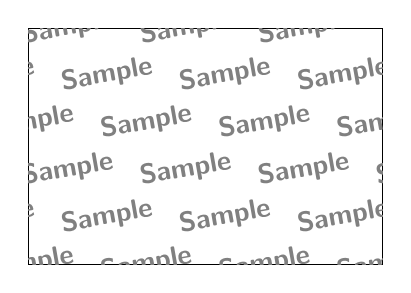
\begin{tikzpicture}
    \draw rectangle++(4.5,3);
    \clip rectangle++(4.5,3);
    \foreach\x in{0,1,2,3,4}{
      \foreach\y in{0,1,2,3,4,5,6}{
        \path(\x*1.5-\y*0.5,\y*0.6)node[rotate=10,text=gray]{\sffamily\bfseries\itshape Sample };
      }
    }
  \end{tikzpicture}
  %% 入れる画像：display.launch.py を起動し、RViz2 に RobotModel と TF を表示した画面と、joint_state_publisher_gui のウィンドウのスクリーンショット
  % eps 画像を貼る場合は includegraphics をお使いください。
  % \includegraphics[width=0.8\linewidth]{tf_viz/rviz.png}
  \caption{RViz2 でロボットのモデルと座標系を表示した例}
  \label{fig:tf-viz-rviz}
\end{figure}

RViz2 でよく使う表示（Display）には、次のようなものがあります。
「Add」の画面の「By topic」タブを使うと、今流れているトピックの中から選んで追加することもできます。

\begin{tablebox}[RViz2 のよく使う表示][tab:tf-viz-displays]
  \begin{tabular}{lp{0.6\linewidth}}
    \toprule
    表示 & 表示するもの \\
    \midrule
    RobotModel & URDF のロボットのモデル \\
    TF & 座標系の位置と向き \\
    LaserScan & LiDAR で測った点（\cmd{sensor\_msgs/msg/LaserScan}） \\
    Image & カメラの画像（\cmd{sensor\_msgs/msg/Image}） \\
    Map & 地図（\ref{sec:practice-slam}節） \\
    Path & 計画した経路 \\
    \bottomrule
  \end{tabular}
\end{tablebox}

\subsection{設定を保存する}

RViz2 を閉じると、設定は消えてしまいます。
メニューの「File」→「Save Config As」で、設定を \cmd{.rviz} という拡張子のファイルに保存しておくと、次からは \cmd{rviz2 -d ファイル名.rviz} で、同じ設定で起動できます。
launch ファイルから起動するときは、\cmd{Node} に \cmd{arguments=['-d', 設定ファイルの場所]} を書きます。

\begin{caution}[VirtualBox で RViz2 が表示されないとき]
  VirtualBox などの仮想マシンでは、3D の表示がうまくいかず、RViz2 の画面が真っ黒になったり、起動してすぐに終了したりすることがあります。
  そのときは、次のように、3D の計算を CPU で行う設定にしてから起動してみましょう。
\begin{lstlisting}[numbers=none, xleftmargin=0pt, framexleftmargin=0pt]
$ export LIBGL_ALWAYS_SOFTWARE=1
$ rviz2
\end{lstlisting}
  表示は遅くなりますが、動くようになることがあります。
\end{caution}

\section*{この章のまとめ}

\begin{itemize}
  \item ロボットでは、本体・センサ・地図など、たくさんの座標系を使います。ROS 2 では、x 軸が前、y 軸が左、z 軸が上で、単位は m と rad です。
  \item tf2 は、座標系どうしの位置関係を \cmd{/tf} と \cmd{/tf\_static} で管理し、どの 2 つの座標系の間でも座標変換を計算してくれます。\cmd{tf2\_echo} や \cmd{view\_frames} で調べられます。
  \item URDF では、ロボットをリンクとジョイントの組み合わせで書きます。
  \item robot\_state\_publisher は、URDF と \cmd{/joint\_states} から座標変換を計算して、tf2 に流します。
  \item RViz2 で、ロボットのモデル・座標系・センサのデータなどを表示できます。設定は \cmd{.rviz} ファイルに保存しておきましょう。
\end{itemize}
